%%%%%%%%%%%%%%%%%%%%%%%%%%%%%%%%%%%%%%%%%%%%%%%%%%%%%%%%%%%%%%%%%%%%%%%%%%%%%%%%
% TUM-Vorlage: Präsentation - Beispiele
%%%%%%%%%%%%%%%%%%%%%%%%%%%%%%%%%%%%%%%%%%%%%%%%%%%%%%%%%%%%%%%%%%%%%%%%%%%%%%%%


%%%%%%%%%%%%%%%%%%%%%%%%%%%%%%%%%%%%%%%%%%%%%%%%%%%%%
%% Folie: Gültigkeit der Masterfolien              %%
%%%%%%%%%%%%%%%%%%%%%%%%%%%%%%%%%%%%%%%%%%%%%%%%%%%%%

%%%%%%%%%%%%%%%%%%%%%%%%%%%%%%%%%%%%%%%%%%%%%%%%%%%%%
%% Folie: Grundlage der Masterfolien               %%
%%%%%%%%%%%%%%%%%%%%%%%%%%%%%%%%%%%%%%%%%%%%%%%%%%%%%

%%%%%%%%%%%%%%%%%%%%%%%%%%%%%%%%%%%%%%%%%%%%%%%%%%%%%
%% Folie: 2-zeilige Überschrift                    %%
%%%%%%%%%%%%%%%%%%%%%%%%%%%%%%%%%%%%%%%%%%%%%%%%%%%%%

\begin{frame}
    \shiftedframetitle{Content}
    
    \begin{enumerate}
    \item Shallow Water Equations model \vspace{0.5cm}
    \item Scope of this thesis\vspace{0.5cm}
    \item Tools\vspace{0.5cm}
    \item Current status\vspace{0.5cm}
    \item TODOs
    \end{enumerate}


%And here are the references:~\cite{bianchi2005understanding}


\end{frame}
\clearpage


%%%%%%%%%%%%%%%%%%%%
%%%%%%%%%%%%%%%%%%%%
\begin{frame}
    \shiftedframetitle{Shallow Water Equations (SWE) model}
    
\begin{multicols}{2}
\begin{itemize}

\item<2->[]
\begin{itemize}
\item derived from mass and momentum conservation laws, and depth averaging \dots %also derived by vertical averaging from the 3d incompressible ns eqs
\vspace{5pt}
\begin{align*}
\begin{bmatrix}[1.5]
h\\
hu\\
hv\\
\end{bmatrix}_t \ + \ 
\begin{bmatrix}[1.5]
uh\\
hu^2 + \frac{1}{2}gh^2\\
huv\\
\end{bmatrix}_x\ &+ \ 
\begin{bmatrix}[1.5]
vh\\
huv\\
hv^2 + \frac{1}{2}gh^2\\
\end{bmatrix}_y = 
\begin{bmatrix}[1.5]
0\\
-gh\frac{\partial b}{\partial x}\\
-gh\frac{\partial b}{\partial y}
\end{bmatrix}\\[1em]
\frac{\partial q}{\partial t} + \dfrac{\partial F(q)}{\partial x} + &\frac{\partial G(q)}{\partial y} = S(q,x,y,t) 
\end{align*}
\vspace{1em}
\item<3-> $ W \ll U,V $\\[0.5em]
\item<4-> $3D\rightarrow 2D$ \\[0.5em]
\item<5-> Applications: {\small Free surface flows, tsunamis prediction, atmospheric flows, \dots} \\[0.5em]
\item<6-> hyperbolic PDE system $\rightarrow$ Riemann Problem and FVM
\end{itemize}
    \vfill\columnbreak
    \vspace*{0.39cm}
\item<1->[]
\begin{figure}
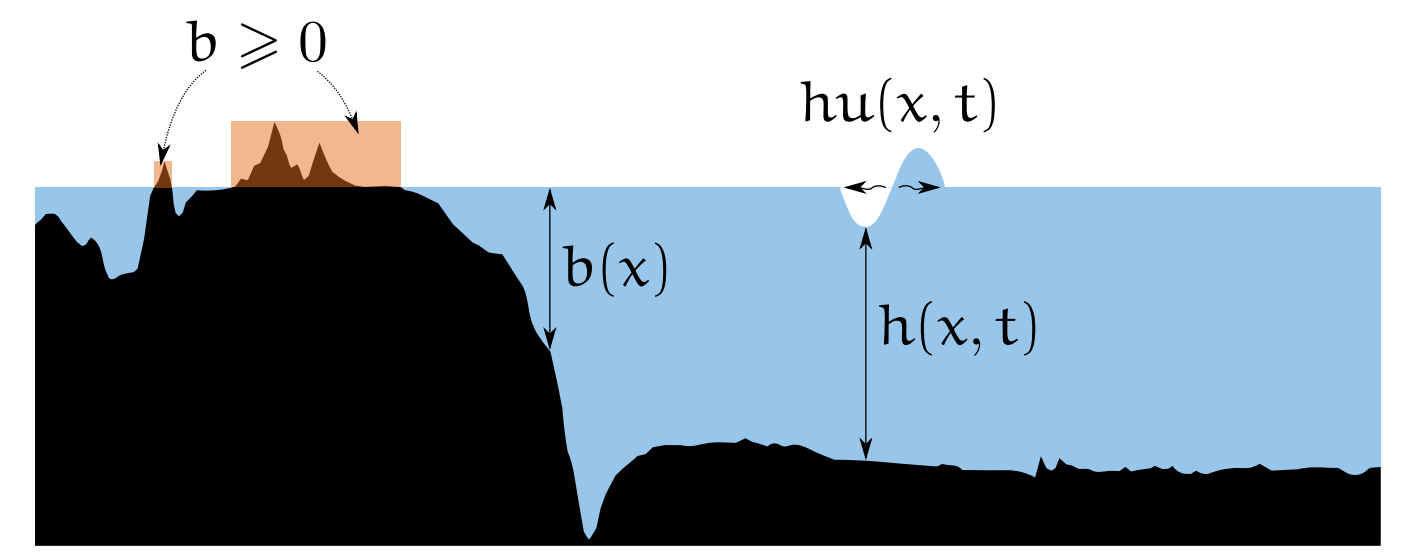
\includegraphics[width=\columnwidth, height=.4\textheight]{./Resources/Images/swe.png}%
\caption{SWE variables schematic \footnote{\url{https://www5.in.tum.de/SWE/lugano2013/swe_anatomy.pdf}}}
\end{figure}
\end{itemize}
\end{multicols}
\end{frame}
\clearpage

%%%%%%%%%%%%%%%%%%%%%%%%%%
%%%%%%%%%%%%%%%%%%%%%%%%%%

\begin{frame}
\shiftedframetitle{Scope of this thesis}

\begin{multicols}{2}
\begin{itemize}
\item<1->[]    
 \hspace{0.35\columnwidth}{\large\textbf{Background}}
 \begin{itemize}
   \setlength\itemsep{2em}
  \item  full description of \textit{shallowFOAM}  solver for 2D SWE \cite{mintgen}
 \item  coupling 2D SWE and 3D RANS solvers $\rightarrow$ development of \textit{shallowInterFOAM} \cite{mintgen}
 \item BSc. Christiaan Osse\footnote{Thesis published during this thesis} implemented \cite{mintgen} with \textit{preCICE}
 \end{itemize}
    
 \vfill\columnbreak

\item<2->[]
\hspace{0.35\columnwidth}{\large\textbf{Goals}}
 \begin{itemize}
    \setlength\itemsep{2em}

 \item<3-> Extend \cite{mintgen} coupling (2D $\Longleftrightarrow$ 3D) as a flexible approach to SWE solvers
 \item<4-> Test Case: 2D SWE solver \& OpenFOAM 
 \item<5-> Coupling \& Mapping data from/to all setups: \vspace{0.4cm}
\begin{table}[]
\begin{tabular}{|llll|}
\hline
Bidirectional & 2D SWE       & - & 2D SWE       \\ \hline
Upstream      & 2D SWE       & - & 3D OpenFOAM \\ \hline
Upstream      & 3D OpenFOAM & - & 2D SWE       \\ \hline
Bidirectional & 3D OpenFOAM & - & 3D OpenFOAM \\ \hline
\end{tabular}
\caption{Mapping setups}
\label{table:1}
\end{table}
\item<6-> \textbf{\textit{Extend preCICE adapter for handling 3D domains}}
\end{itemize}
\end{itemize}
\end{multicols}


\end{frame}


%%%%%%%%%%%%%%%%%%
%%%%%%%%%%%%%%%%%%

\begin{frame}
	\shiftedframetitle{Tools}
 	
\begin{multicols}{2}
\begin{itemize}
 \setlength\itemsep{10pt}

\item<2->[]
\textbf{Shallow Water Equations Solver - Wave-propagation method.}
\begin{itemize}
\vspace{5pt}
 \setlength\itemsep{6pt}
\item Modified Wave-Propagation Method $\rightarrow$ \textit{F-Wave} \cite{levequeArticle}
\item Developed at SCCS\footnote{\url{https://github.com/TUM-I5/SWE}}
\item Written in C++
\item 2-D
\end{itemize}

\item<3->[]
\textbf{\textit{interFOAM}\footnote{\url{https://openfoamwiki.net/index.php/InterFoam}} - OpenFoam Multiphase Navier-Stokes Solver}
\begin{itemize}
\vspace{5pt}
 \setlength\itemsep{6pt}
\item VoF (Volume of Fluid) method
\item immiscible fluids (gas and liquid)
\item 3-D
\end{itemize}

\vfill\columnbreak
\item<4->[]
\textbf{preCICE\footnote{\url{https://github.com/precice}} - Open Source coupling library for partitioned multi-physics simulations}
\begin{itemize}
\vspace{5pt}
\item coupling \& mapping {\tiny (see table \ref{table:1})}
\begin{itemize}
\item two domains on \textit{same} dimensions/solvers
\item two domains on \textit{different} dimensions/solvers
\end{itemize}
\end{itemize}
\end{itemize}

\end{multicols}

\end{frame}

%%%%%%%%%%%%%%%%%%
%%%%%%%%%%%%%%%%%%


\begin{frame}
\shiftedframetitle{Current Status}
\begin{multicols}{2}
\begin{itemize}
\item<1->[]
{\renewcommand{\arraystretch}{2.5} %<- modify value to suit your needs
\begin{table}[]
\begin{tabular}{ cl }
{\large\textbf{Progress}} & {\large\hspace{5pt} \textbf{Implementation}}\\

\includegraphics[scale=0.5]{./Resources/Images/bar1.png} & \hspace{5pt}Bidirectional 2D SWE - 2D SWE  \\ 
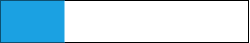
\includegraphics[scale=0.5]{./Resources/Images/bar2.png} &\hspace{5pt} Upstream 2D SWE - 3D OF \\ 
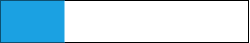
\includegraphics[scale=0.5]{./Resources/Images/bar2.png} &\hspace{5pt} Upstream 3D OF - 2D SWE \\ 
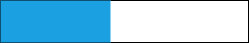
\includegraphics[scale=0.5]{./Resources/Images/bar3.png} & \hspace{5pt} Bidirectional 3D OF - 3D OF \\
\end{tabular}

\end{table}
}

\vfill\columnbreak

\item<2->[] \hspace{0.35\columnwidth}{\Large\textbf{Challenges}}\\[2.5cm]
\item<3->[] {\Large\hspace{0.23\columnwidth}Boundary Conditions!!}
\begin{itemize}
 \setlength{\itemindent}{3.5cm}
\vspace{0.5cm}
\item<4-> Inflow / Outflow 
\item<4-> Dirchlet / Neumann / Robin
\end{itemize}
\end{itemize}
\end{multicols}
\end{frame}


%%%%%%%%%%%%%%%%%%
%%%%%%%%%%%%%%%%%%
\begin{frame}
\shiftedframetitle{Current Status}
\vspace{-0.5cm}
{\large \hspace{3mm} Special Considerations}

\end{frame}

%%%%%%%%%%%%%%%%%%
%%%%%%%%%%%%%%%%%%
\begin{frame}
\shiftedframetitle{Current Status}
\vspace{-0.5cm}
{\large \hspace{3mm} Some Results}
add results
\end{frame}

%%%%%%%%%%%%%%%%%%
%%%%%%%%%%%%%%%%%%
\begin{frame}
\shiftedframetitle{TODOs}

\begin{figure}
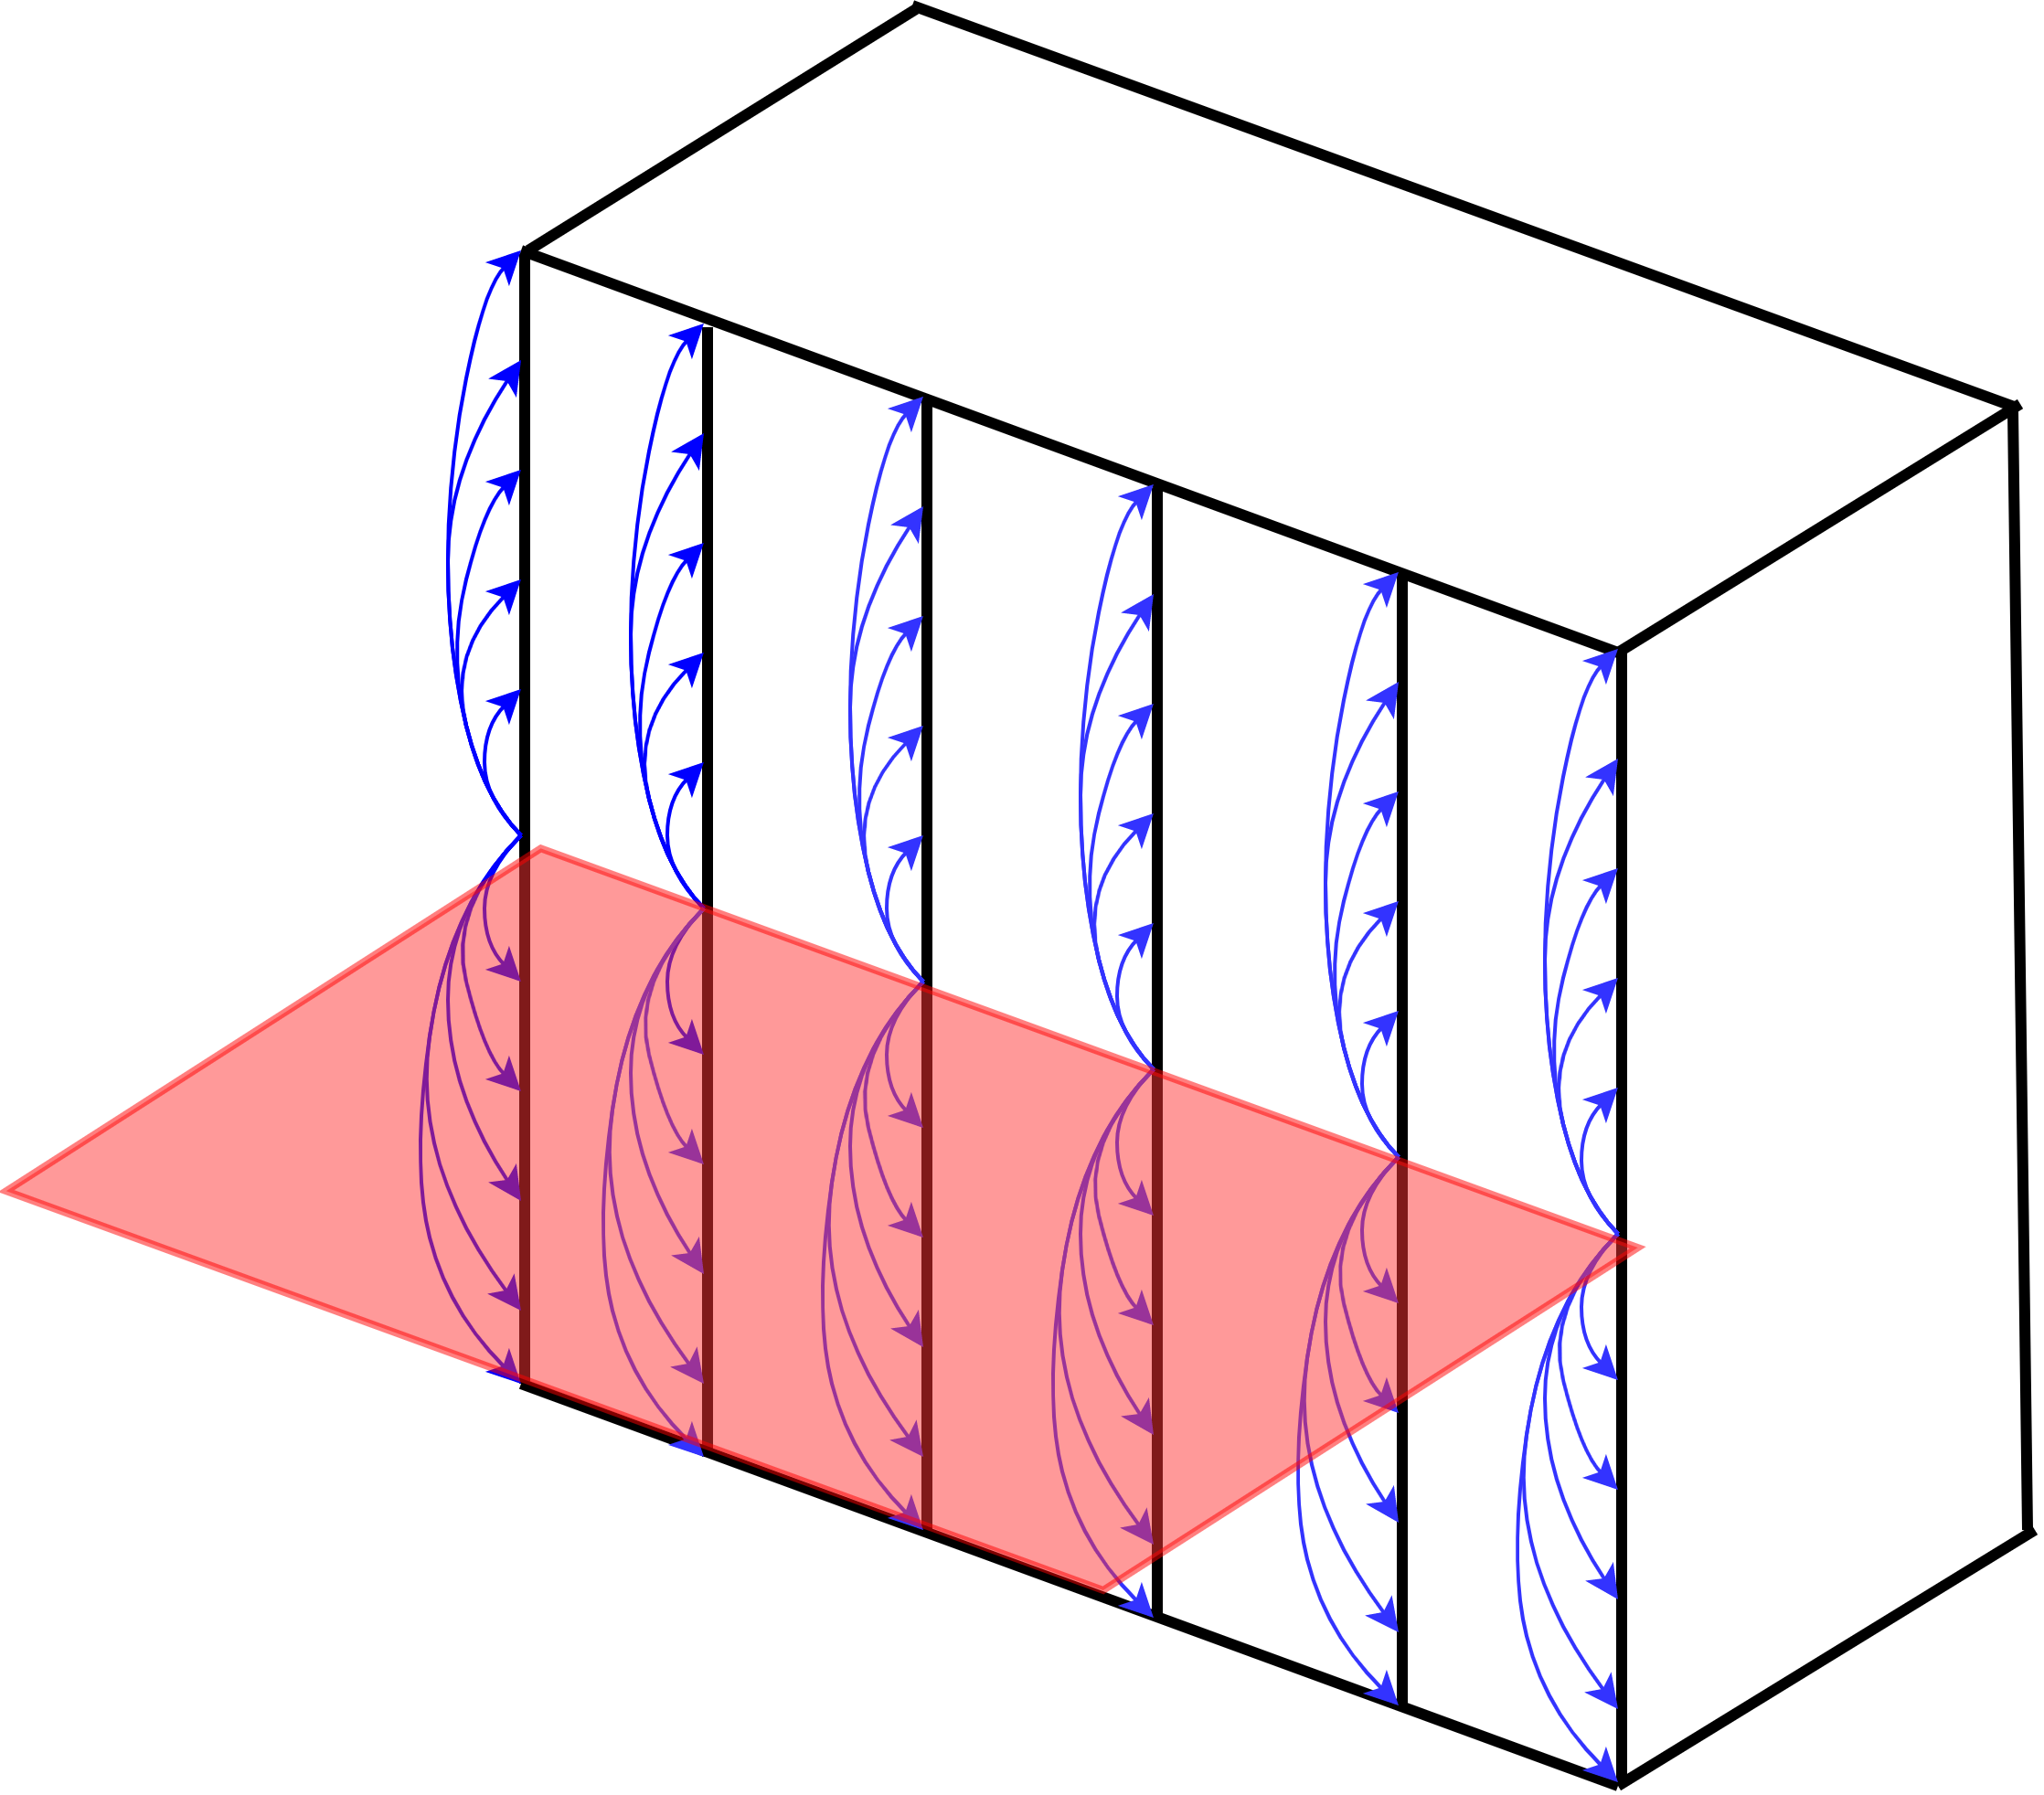
\includegraphics[scale=0.5]{./Resources/Images/mapping23.png}%
\caption{mapping 2D to 3D}
\end{figure}

\end{frame}


%%%%%%%%%%%%%%%%%%
%%%%%%%%%%%%%%%%%%
\begin{frame}
\shiftedframetitle{TODOs}

\begin{figure}
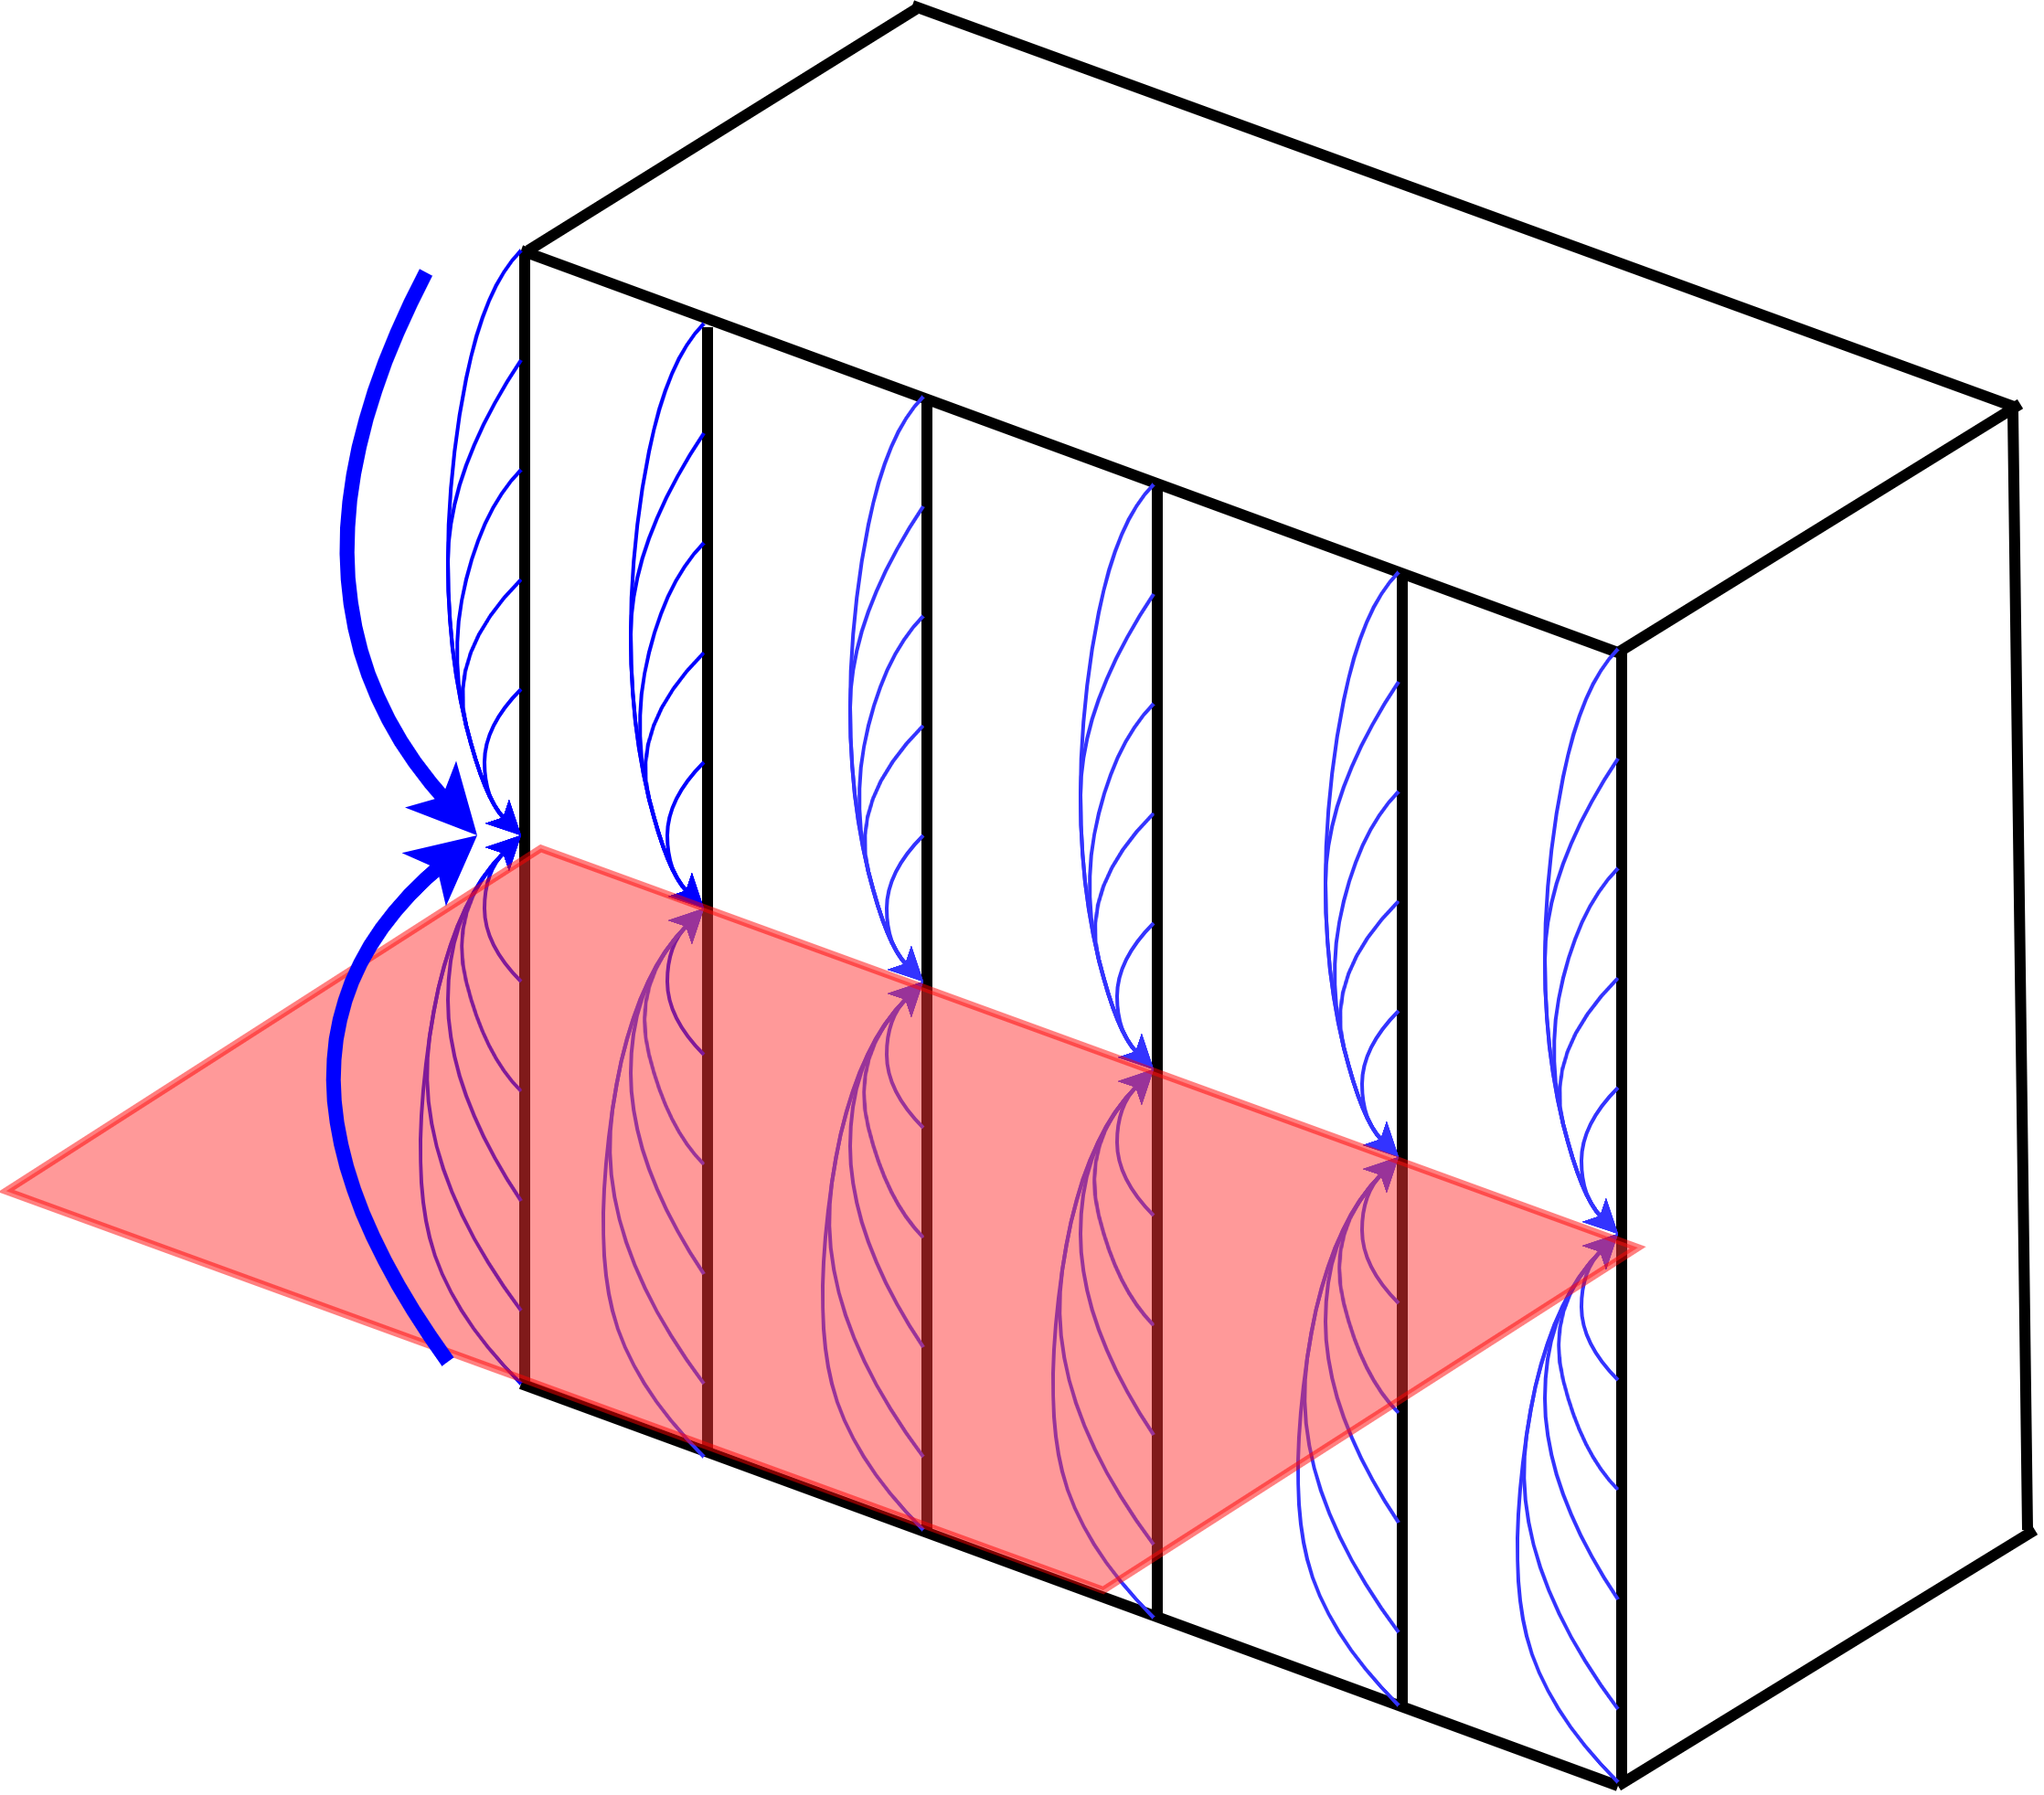
\includegraphics[scale=0.5]{./Resources/Images/mapping32.png}%
\caption{mapping 3D to 2D}
\end{figure}

\end{frame}


%%%%%%%%%%%%%%%%%%%
%% Folie: Farben %%
%%%%%%%%%%%%%%%%%%%
\begin{frame}
    \shiftedframetitle{Farben}
    
Als erstes soll mit schwarz und weiß gearbeitet werden.\newline
Für Aufwändigere Darstellungen sind Farben mit Bedacht und in möglichst
geringem Umfang einzusetzen.

In diesem Folienmaster ist die Farbpalette festgelegt.

{
    \renewcommand{\arraystretch}{1.2} % skaliert die Tabellen mit Farbfeldern

    Zuerst mit den Primärfarben arbeiten.

    \setlength{\fboxsep}{-1pt} \setlength{\fboxrule}{1pt} % fbox/framebox konfigurieren

    \vspace*{-5mm}
    \begin{tabularx}{\textwidth}{@{} l @{\hspace{4mm}} l @{\hspace{4mm}} l}
        \crule[TUMBlau]{24mm}{6mm}
        & \crule[black]{24mm}{6mm}
        & \fbox{\crule[white]{24mm}{6mm}}
    \end{tabularx}

    \vspace*{-5mm}
    Für z.B. komplexe Diagramme stehen noch Sekundärfarben zur Verfügung.

    \vspace*{-5mm}
    \begin{tabularx}{\textwidth}{@{} l @{\hspace{4mm}} l @{\hspace{4mm}} l @{\hspace{4mm}} l}
        \crule[TUMBlauDunkel]{24mm}{6mm}
        & \crule[TUMBlauMittel]{24mm}{6mm}
        & \crule[TUMBlauHell]{24mm}{6mm}
        & \crule[TUMGrau]{24mm}{6mm}
    \end{tabularx}

    \vspace*{-5mm}
    Bei weiterer Komplexität oder zusätzlichen Markierungen:

    \vspace*{-5mm}
    \begin{tabularx}{\textwidth}{@{} l @{\hspace{4mm}} l @{\hspace{4mm}} l }
        \crule[TUMOrange]{24mm}{6mm}
        & \crule[TUMGruen]{24mm}{6mm}
        & \crule[TUMElfenbein]{24mm}{6mm}
    \end{tabularx}
}

\end{frame}
\clearpage


%%%%%%%%%%%%%%%%%%
%% Folie: Texte %%
%%%%%%%%%%%%%%%%%%
\begin{frame}
    \shiftedframetitle{Texte}
 
Kurze und knappe Texte, Fließtexte linksbündig, kein Blocksatz \\[\baselineskip]

Beispiel:\newline
Tem soluptam, nisi as verum ereprehendam at acculpa quidisq uissit volupta
tusdant utem as etur, odi odis es doluptiae dem nimaion con nossinctenis pora
quam voloria consenimus blabore everfer epeliquo maio etur.

\end{frame}
\clearpage




%%%%%%%%%%%%%%%%%%%%%%%%%%%%%%
% Folie: Bilder - Allgemein %%
%%%%%%%%%%%%%%%%%%%%%%%%%%%%%%
\begin{frame}
    \shiftedframetitle{Bilder -- Allgemein}
    
schlichte Darstellung von Informationen \\[\baselineskip]

reduzierte Farben \\[\baselineskip]

Rahmen und Überlagerungen nach Möglichkeit vermeiden \\[\baselineskip]

    
\end{frame}
\clearpage


%%%%%%%%%%%%%%%%%%%%%%%%%
% Folie: Bilder - Zwei %%
%%%%%%%%%%%%%%%%%%%%%%%%%
\begin{frame}
    \shiftedframetitle{Bilder}
    
Bildbeschreibung\newline
oberer Bildrand: Begrenzung durch Text\\[\baselineskip]

\mbox{
\includegraphics[height=.5\paperheight, trim=0cm 14cm 0cm 0cm, clip=true]{./Resources/Images/SternenhimmelHochkant.jpg}}%
\hspace{6.5mm}%
\mbox{
\includegraphics[height=.5\paperheight, trim=0cm 14cm 0cm 0cm, clip=true]{./Resources/Images/SternenhimmelHochkant.jpg}}

\end{frame}
\clearpage


%%%%%%%%%%%%%%%%%%%%%%%%%%%%%%%%%%%%%%%
% Folie: Bilder - Zweispaltige Seite %%
%%%%%%%%%%%%%%%%%%%%%%%%%%%%%%%%%%%%%%%
\begin{frame}
    \shiftedframetitle{Bilder}

\begin{multicols}{2}
    \textbf{Überschrift 2}\newline
    Hier steht ein einleitender oder beschreibender Fließtext und nach Wunsch
    eine Aufzählung.

    Punkt 1

    Punkt 2

    Punkt 3

    Punkt 4
    \vfill\columnbreak
    
\includegraphics[width=\columnwidth, height=.7\textheight]{./Resources/Images/SternenhimmelHochkant.jpg}%
\end{multicols}
    
\end{frame}
\clearpage


%%%%%%%%%%%%%%%%%%%%%%%%%%%%%%
% Folie: Bilder - Textbreit %%
%%%%%%%%%%%%%%%%%%%%%%%%%%%%%%
\begin{frame}
    \shiftedframetitle{Bilder}

Bildbeschreibung\newline
oberer Bildrand: Begrenzung durch Text\\[\baselineskip]


\includegraphics[width=\textwidth, height=.55\textheight]{./Resources/Images/SternenhimmelQuer.jpg}%

\end{frame}
\clearpage

%%%%%%%%%%%%%%%%%%%%%%%%%%%%%%%%%%%%%%%%%%%%%%%%%
% Folie: Bilder - seitenbreit mit Beschreibung %%
%%%%%%%%%%%%%%%%%%%%%%%%%%%%%%%%%%%%%%%%%%%%%%%%%
\begin{frame}
    \shiftedframetitle{Bilder}

    Bildbeschreibung\newline
    oberer Bildrand: Begrenzung durch Text

\vspace*{-3mm}
\begin{minipage}[t][0cm]{\paperwidth}%
\hspace*{-\PraesentationSeitenrand}%

\includegraphics[width=\paperwidth]{./Resources/Images/SternenhimmelQuer.jpg}
\end{minipage}
    
\end{frame}
\clearpage

%%%%%%%%%%%%%%%%%%%%%%%%%%%%%%%%%%%%%%%%%%%%%%%%%%%%
% Folie: Nicht Format füllende Bilder %%
%%%%%%%%%%%%%%%%%%%%%%%%%%%%%%%%%%%%%%%%%%%%%%%%%%%%
\begin{frame}
    \shiftedframetitle{Nicht Format füllende Bilder}
    
    Weißer bzw. transparenter Hintergrund\newline
    mit genug Freiraum anordnen


\begin{textblock*}{0.4\paperwidth}[0,1](0cm, \textheight - \PraesentationSeitenrand)%
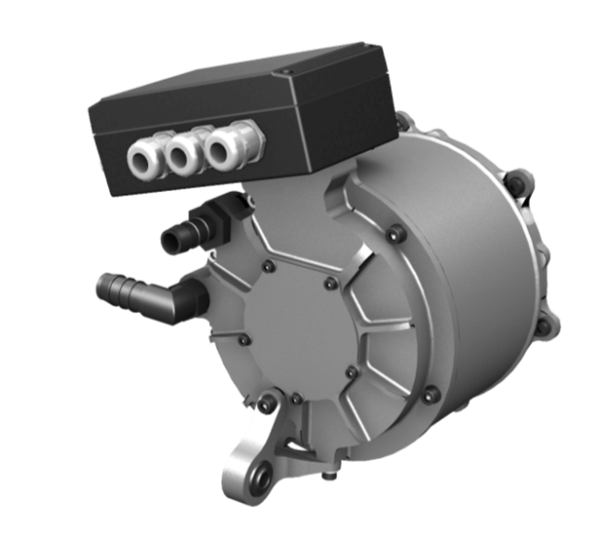
\includegraphics[width=0.4\paperwidth]{./Resources/Presentation/Images/Motor.png}
\end{textblock*}

\begin{textblock*}{0.6\paperwidth}[1,1](\textwidth + \PraesentationSeitenrand, \textheight - \PraesentationSeitenrand)%
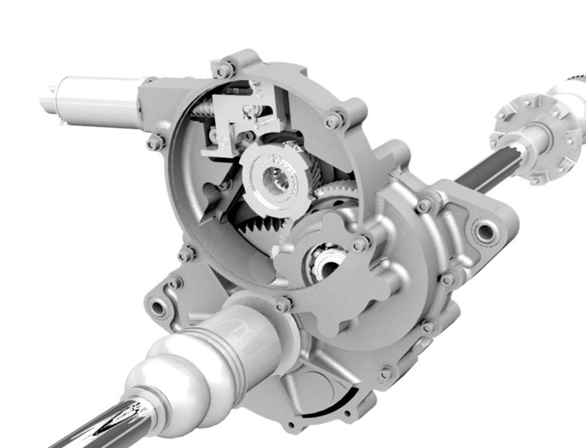
\includegraphics[width=0.6\paperwidth]{./Resources/Presentation/Images/Getriebe.png}
\end{textblock*}

\end{frame}
\clearpage


%%%%%%%%%%%%%%%%%%%%%%%%%%%%%%%%%%
% Folie: Bilder - formatfüllend %%
%%%%%%%%%%%%%%%%%%%%%%%%%%%%%%%%%%
\begin{frame}
    \shiftedframetitle{Bilder Format füllend -- maximale Bildgröße}

\begin{minipage}[t][0cm]{\paperwidth}%
\hspace*{-\PraesentationSeitenrand}%

\includegraphics[width=\textwidth]{./Resources/Images/SternenhimmelQuer.jpg}
\end{minipage}
    
\end{frame}
\clearpage

%%%%%%%%%%%%%%%%%%%%%%%%%%%%%%%%%%%%%%%%%%%%%%%%%%%%%
%% Folie: Nicht Format füllende Bilder %%
%%%%%%%%%%%%%%%%%%%%%%%%%%%%%%%%%%%%%%%%%%%%%%%%%%%%%
\begin{frame}
    \shiftedframetitle{Nicht Format füllende Bilder}
    
Alternativ mit formatfüllendem Hintergrund: Weiß 5\% dunkler\newline
Beschriftungen können zusätzlich neben den Bildern angebracht werden

\begin{textblock*}{\paperwidth}[0,0](0cm, .4\textheight)%
Bilderklärung
\end{textblock*}

\begin{textblock*}{\paperwidth}[1,0](\textwidth, .4\textheight)%
\raggedleft%
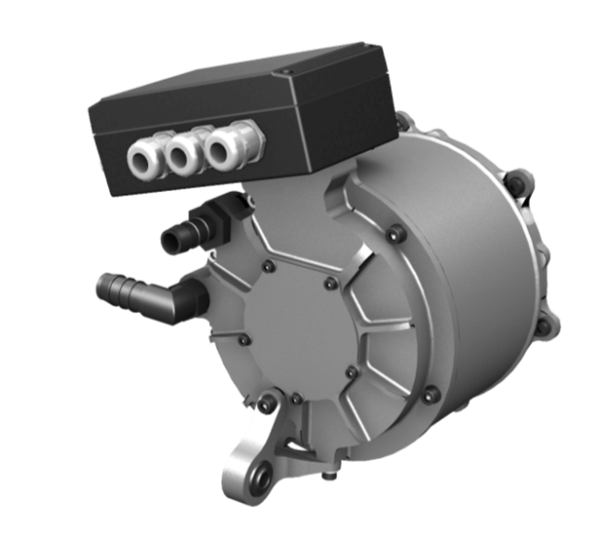
\includegraphics[height=0.5\textheight]{./Resources/Presentation/Images/Motor.png}
\end{textblock*}

\end{frame}
\clearpage


%%%%%%%%%%%%%%%%%%%%%%%%%%%%%%%%%%%%%%%%%%%%%%%%%%%%
% Folie: Tabelle - Ohne Rand 					   %%
%%%%%%%%%%%%%%%%%%%%%%%%%%%%%%%%%%%%%%%%%%%%%%%%%%%%
\begin{frame}
    \shiftedframetitle{Tabelle -- Beispiel 1}
    
Tabelle ohne Farbe und kein Rand \\
innerer Seitenrand links 0 cm, um Faktor 1,75 skalierte Tabelle (für genug Zeilenabstand)

\raggedright
{
    \vspace*{0.3pt}
    \renewcommand{\arraystretch}{1.75} % skaliert die Tabelle auf die gewünschte Größe
    \begin{tabularx}{\textwidth}{@{} l @{\hspace{38.7mm}} l}
        Ø - Strecke & 39 km/Tag (14.360 km/Jahr) \\
        Ø - Geschwindigkeit & 25 km/h \\
        Ø - Verfügbare Ladezeit & 22 h/Tag \\
        Kosten   & Kleinwagen mit Verbrennungsmotor \\
        Einsatzgebiet   &  Stadt und Umland
    \end{tabularx}
}
\end{frame}


%%%%%%%%%%%%%%%%%%%%%%%%%%%%%%%%%%%%%%%%%%%%%%%%%%%%%
%% Folie: Tabelle - Mit Rand                       %%
%%%%%%%%%%%%%%%%%%%%%%%%%%%%%%%%%%%%%%%%%%%%%%%%%%%%%
\begin{frame}
    \shiftedframetitle{Tabelle -- Beispiel 2}
    
Tabelle ohne Farbe und mit Rand\\
automatische Zelleninnenabstände, um Faktor 1,75 skalierte Tabelle (für genug Zeilenabstand)

\raggedright
{
    \vspace*{0.3pt}
    \renewcommand{\arraystretch}{1.75} % skaliert die Tabelle auf die gewünschte Größe
    \begin{tabularx}{\textwidth}{| l @{\hspace{38.7mm}} | X |}
        \hline
        Ø - Strecke & 39 km/Tag (14.360 km/Jahr) \\ \hline
        Ø - Geschwindigkeit & 25 km/h \\ \hline
        Ø - Verfügbare Ladezeit & 22 h/Tag \\ \hline
        Kosten   & Kleinwagen mit Verbrennungsmotor \\ \hline
        Einsatzgebiet   &  Stadt und Umland \\ \hline
    \end{tabularx}
}
\end{frame}

\clearpage


%%%%%%%%%%%%%%%%%%%%%%%%%%%%%%%%%%%%%%%%%%%%%%%%%%%%%
%% Folie: Diagramme - Beispiel 1                   %%
%%%%%%%%%%%%%%%%%%%%%%%%%%%%%%%%%%%%%%%%%%%%%%%%%%%%%
\begin{frame}
    \shiftedframetitle{Diagramme -- Beispiel 1}

%Nach Möglichkeit linksbündig bleiben \\
%Unnötige Striche und Balken vermeiden

\begin{center}%
    \vspace*{-1cm}
   \begin{tikzpicture}
        \begin{axis}[
                % kein Abstand zwischen Balken:
                xbar=0,
                draw opacity=0,
                bar width=14,
                axis x line=none,
                axis line style={transparent},
                every tick/.style={transparent},
                xmin=0,
                width=\textwidth,
                height=.6\textheight,
                enlarge y limits=0.15,
                symbolic y coords={Kategorie 4,Kategorie 3,Kategorie 2,Kategorie 1},
                ytick=data,
                legend image code/.code={\draw[draw=none] (0cm,-0.12cm) rectangle (0.29cm,0.17cm);}, % Legenden-Symbol  
                legend columns=3,
                reverse legend,
                legend style={
                    fill=none,
                    draw=none,
                    /tikz/every odd column/.append style={column sep=0.07cm}, % Abstand zwischen Legenden-Symbol und Text
                    /tikz/every even column/.append style={column sep=0.8cm} % Abstand zwischen den Legendeneinträgen
                 },
                 legend to name=PraesentationDiagrammHorizontalLegende
            ]
            
            \addlegendentry{Datenreihe 3}
            \addlegendentry{Datenreihe 2}
            \addlegendentry{Datenreihe 1}
            
            \addplot[color=TUMBlauMittel, fill=TUMBlauMittel] coordinates {
                (1.2,Kategorie 1)
                (1.6,Kategorie 2)
                (2.2,Kategorie 3)
                (3.4,Kategorie 4)
            };
            
            \addplot[color=TUMBlauHell, fill=TUMBlauHell] coordinates {
                (1.5,Kategorie 1)
                (3.0,Kategorie 2)
                (1.0,Kategorie 3)
                (2.0,Kategorie 4)
            };
                
            \addplot[color=TUMBlauDunkel, fill=TUMBlauDunkel] coordinates {
                (3.0,Kategorie 1)
                (2.0,Kategorie 2)
                (2.5,Kategorie 3)
                (3.0,Kategorie 4)
            };
        \end{axis}
    \end{tikzpicture}

    \vspace*{-5mm}
    \ref*{PraesentationDiagrammHorizontalLegende}%
\end{center}
\end{frame}
\clearpage


%%%%%%%%%%%%%%%%%%%%%%%%%%%%%%%%%%%%%%%%%%%%%%%%%%%%%
%% Folie: Diagramme                                %%
%%%%%%%%%%%%%%%%%%%%%%%%%%%%%%%%%%%%%%%%%%%%%%%%%%%%%
\begin{frame}
    \shiftedframetitle{Diagramme}

\begin{center}
    \begin{tikzpicture}
        \begin{axis}[
                ybar=9.5,
                bar width=27.1,
                axis line style={transparent},
                every tick/.style={transparent},
                enlarge x limits=0.145, % X-Achse skalieren
                clip limits=true,
                ymin=0,
                ymax=6,
                width=\textwidth,
                height=.65\textheight,
                symbolic x coords={Kategorie 1,Kategorie 2,Kategorie 3,Kategorie 4},
                xticklabels={Kategorie 1,Kategorie 2,Kategorie 3,Kategorie 4},
                xtick=data,
                ytick={0,1,2,3,4,5,6},
                every tick label/.append style={font=\fontsize{13}{14}\selectfont},
                ymajorgrids,
                legend image code/.code={\draw[draw=none] (0cm,-0.12cm) rectangle (0.29cm,0.17cm);}, % Legenden-Symbol  
                legend columns=3,
                reverse legend,
                legend style={
                    font={\usebeamerfont{footnote}},
                    fill=none,
                    draw=none,
                    /tikz/every odd column/.append style={column sep=0.07cm}, % Abstand zwischen Legenden-Symbol
                    /tikz/every even column/.append style={column sep=0.8cm} % Abstand zwischen den Legendeneinträgen
                 },
                legend to name=PraesentationDiagrammVertikalLegende
            ]
            
            \addlegendentry{Datenreihe 3}        
            \addlegendentry{Datenreihe 2}    
            \addlegendentry{Datenreihe 1}    
            
            \addplot[color=TUMBlauDunkel, fill=TUMBlauDunkel] coordinates {
                (Kategorie 1,4.2)
                (Kategorie 2,2.5)
                (Kategorie 3,3.5)
                (Kategorie 4,4.5)
            };
            
            \addplot[color=TUMBlauHell, fill=TUMBlauHell] coordinates {
                (Kategorie 1,2.3)
                (Kategorie 2,4.5)
                (Kategorie 3,1.8)
                (Kategorie 4,2.8)
            };
            
            \addplot[color=TUMBlauMittel, fill=TUMBlauMittel] coordinates {
                (Kategorie 1,2.0)
                (Kategorie 2,2.0)
                (Kategorie 3,3.0)
                (Kategorie 4,5.0)
            };        
        \end{axis}
    \end{tikzpicture}

    \vspace*{-5mm}
    \ref*{PraesentationDiagrammVertikalLegende}%
\end{center}
\end{frame}
\clearpage

